%\documentclass[a4paper,eqsecnum,twoside,aps,floatfix,notitlepage]{revtex4}

\documentclass[amsmath,amssymb,12pt,eqsecnum]{revtex4}
\usepackage{graphicx,float,subfloat}
\usepackage[breaklinks, colorlinks, citecolor=blue]{hyperref}
\usepackage{bm}% bold math
\linespread{1}
\usepackage{subfigure}
\usepackage{hyperref}

\newcommand{\Planck}{{\textit{Planck }}}
\newcommand{\SPT}{{\textit{SPT }}}
\newcommand{\CFHTLenS}{{\textit{CFHTLenS }}}
\newcommand{\CoRE}{{\textit{CoRE }}}
\newcommand{\WMAP}{{\textit{WMAP }}}
\newcommand{\Euclid}{{{\it Euclid}}}
\newcommand{\CAMB}{{\tt{CAMB }}}
\newcommand{\MGCAMB}{{\tt{MGCAMB }}}

%\newcommand{\vphi}[0]{{\color{green}{\delta\phi}}}
%\newcommand{\dlg}[0]{{\color{red}{\lp g}}}
\newcommand{\vphi}[0]{\delta\phi}
\newcommand{\lpa}[0]{\lp A}
\newcommand{\dlg}[0]{\lp g}

\newcommand{\depg}[0]{\ep g}
\newcommand{\virt}[0]{\hat{\delta}}
\newcommand{\Dvphi}[1]{\nabla_{#1}\vphi}
\newcommand{\DDvphi}[2]{\nabla_{#1}\nabla_{#2}\vphi}

\newcommand{\Dvvphi}[1]{\nabla_{#1}\virt\vphi}
\newcommand{\DDvvphi}[2]{\nabla_{#1}\nabla_{#2}\virt\vphi}

\newcommand{\tmat}[4]{\left( \begin{array}{cc} #1 & #2 \\ #3 & #4 \end{array}\right)}
\newcommand{\expec}[1]{\left\langle #1\right\rangle}
\newcommand{\half}[0]{\frac{1}{2}}
\newcommand{\cs}[3]{\Gamma^{#1}_{\,\,\,\, #2#3}}

\newcommand{\pd}[2]{\frac{\partial #1}{\partial #2}}
\newcommand{\ld}[0]{\mathcal{L}}
\newcommand{\md}[0]{\mathcal{M}}
\newcommand{\dd}[0]{\textrm{d}}
\newcommand{\defn}[0]{\equiv}
\newcommand{\diag}[0]{\textrm{diag}}
\newcommand{\qsubrm}[2]{{#1}_{\scriptsize{\textrm{#2}}}}
\newcommand{\qsuprm}[2]{{#1}^{\scriptsize{\textrm{#2}}}}
\newcommand{\qsubprm}[3]{{#1}^{\scriptsize{\textrm{#2}}}_{\scriptsize{\textrm{#3}}}}
 \newcommand{\subsm}[2]{{#1}_{\scriptscriptstyle{#2}}}

\newcommand{\supsm}[2]{{#1}^{\scriptscriptstyle{#2}}}
\newcommand{\symmb}[0]{\varrho}
\newcommand{\AW}[0]{A_{\mathcal{W}}}
\newcommand{\BW}[0]{B_{\mathcal{W}}}
\newcommand{\CW}[0]{C_{\mathcal{W}}}
\newcommand{\DW}[0]{D_{\mathcal{W}}}
\newcommand{\EW}[0]{E_{\mathcal{W}}}

\newcommand{\AP}[0]{A_{\mathcal{P}}}
\newcommand{\BP}[0]{B_{\mathcal{P}}}
\newcommand{\CP}[0]{C_{\mathcal{P}}}
\newcommand{\DP}[0]{D_{\mathcal{P}}}
\newcommand{\EP}[0]{E_{\mathcal{P}}}
\newcommand{\FP}[0]{F_{\mathcal{P}}}
\newcommand{\GP}[0]{G_{\mathcal{P}}}

\newcommand{\sol}[0]{\ld_{\scriptscriptstyle\{2\}}}

\newcommand{\tis}[0]{ {\theta}^{\scriptscriptstyle\rm{S}}}
\newcommand{\tisdot}[0]{ {\dot{\theta}}^{\scriptscriptstyle\rm{S}}}
\newcommand{\pis}[0]{ {\Pi}^{\scriptscriptstyle\rm{S}}}
\newcommand{\xis}[0]{ {\xi}^{\scriptscriptstyle\rm{S}}}
\newcommand{\xisdot}[0]{ {\dot{\xi}}^{\scriptscriptstyle\rm{S}}}
\newcommand{\xisddot}[0]{ {\ddot{\xi}}^{\scriptscriptstyle\rm{S}}}
\newcommand{\xisdddot}[0]{ {\dddot{\xi}}^{\scriptscriptstyle\rm{S}}}
\newcommand{\lcdm}[0]{$\Lambda$CDM}

\newcommand{\coup}[0]{\mathcal{Q}}
\newcommand{\vmkin}[0]{\mathcal{K}}



\newcommand{\newchap}[2]{\chapter{#1}
\markboth{\MakeUppercase{Chapter \thechapter.\ #2}}{}}
\newcommand{\nphiu}[1]{\nabla^{#1}\phi}
\newcommand{\nphid}[1]{\nabla_{#1}\phi}

\newcommand{\gbm}[1]{\bm{#1}}
\newcommand{\rbm}[1]{{\bf{#1}}}
\newcommand{\ci}[0]{\textrm{i}}
%\newcolumntype{V}{>{\centering\arraybackslash} m{.4\linewidth} }
\newcommand{\kin}[0]{{\mathcal{X}}}
\newcommand{\hct}[0]{\mathcal{H}}
\renewcommand{\figurename}{Figure}
\newcommand{\ep}[0]{{ {\delta}_{\scriptscriptstyle{\rm{E}}}}}
\newcommand{\lp}[0]{{ {\delta}_{\scriptscriptstyle{\rm{L}}}}}
\def\be{\begin{equation}}
\def\ee{\end{equation}}
\def\bea{\begin{eqnarray}}
\def\eea{\end{eqnarray}}
\def\bse{\begin{subequations}}
\def\ese{\end{subequations}}
\newcommand{\lied}[1]{\pounds_{#1}}

\newcommand{\sech}[0]{\textrm{ sech}}
% Planck style says this should be Fig. 1
\newcommand{\fref}[1]{{Fig.~\ref{#1}}}
\newcommand{\tref}[1]{{Table \ref{#1}}}
\newcommand{\secref}[1]{{section \ref{#1}}}
\newcommand{\Secref}[1]{{Section \ref{#1}}}
% PUT CATCH ON THE END OF SQUARE-ROOT SYMBOLS
\newcommand{\rsbb}[2]{#1_{\mathbb{#2}}}

\newcommand{\dg}[0]{\delta g}
\let\oldsqrt\sqrt
% it defines the new \sqrt in terms of the old one
\def\sqrt{\mathpalette\DHLhksqrt}
\def\DHLhksqrt#1#2{%
\setbox0=\hbox{$#1\oldsqrt{#2\,}$}\dimen0=\ht0
\advance\dimen0-0.2\ht0
\setbox2=\hbox{\vrule height\ht0 depth -\dimen0}%
{\box0\lower0.4pt\box2}}

\newcommand{\sbm}[2]{#1_{\mathbb{#2}}}

\newcommand{\comment}[1]{{\color{red}[#1]}}

 
\begin{document}

\title{Shaping the chameleon}
\author{Jonathan A. Pearson}
\email{j.pearson@nottingham.ac.uk}
\affiliation{School of Physics \& Astronomy, University of Nottingham, Nottingham, NG7 2RD, U.K.}	
\date{\today}

\maketitle


\tableofcontents

 
 
 
\section{Introduction}

The source density is $\rho(\rbm{x})$.  Different geometrical shapes of this source (such as ellipses, rectangles, triangles, etc) will yield different gravitational potentials, and will alter how the chameleon scalar responds.

The effective potential for the chameleon is
\bea
\label{eff-pot-cham}
\qsubrm{V}{eff} = \frac{\Lambda^5}{\phi} + \frac{\rho(\rbm{x})}{M}\phi + \half m^2\left( \phi - \phi_{\infty}\right)^2.
\eea
The field equations governing the chameleon scalar and gravitational potential are
\bse
\label{eq:eom-cham-}
\bea
\label{eq:eom-cham-phi}
\nabla^2\phi = \frac{\dd \qsubrm{V}{eff}}{\dd\phi},
\eea
\bea
\label{eq:eom-cham-grav}
\nabla^2\Phi = - \rho(\rbm{x})/2\qsubrm{M}{pl}^2.
\eea
\ese
The force on a test particle, due to the gravitational and chameleon scalars are given by
\bse
\bea
\label{cham_force}
\rbm{F}_{(\phi)} = - \tfrac{1}{M}\nabla\phi,
\eea
\bea
\label{grav_force}
\rbm{F}_{(\Phi)} = - \nabla\Phi.
\eea
\ese
The idea is to obtain the source-shape that maximises the force that a test particle will feel, that cannot be explained by forces of a purely gravitational origin.

We construct the function $\rho(\rbm{x})$ such that
\bea
\rho = \left\{ \begin{array}{cc} \rho_0 & \mbox{inside object}, \\ 0 & \mbox{outside object}. \end{array}\right.
\eea

\section{Explanation of numerical methods}
Except in the simplest scenarios and geometries, solutions to the field equations (\ref{eq:eom-cham-}) can only be found with numerical methods. The intermediary  aim is to understand the features in the field of forces due to the chameleon scalar, obtained by applying (\ref{cham_force}) to  solutions of (\ref{eq:eom-cham-phi}), as well as understanding the properties of the gravitational force (\ref{grav_force}). We treat and obtain the chameleon and gravitational forces very differently. 

The equations   implemented by our numerical methods are dimensionless. We set
\bse
\bea
\phi = \sqrt{M\Lambda^5}\tilde{\phi},\qquad
\Phi = \frac{M}{\qsubrm{M}{Pl}^2}\sqrt{M\Lambda^5}\tilde{\Phi},
\eea
\bea
x^{\mu} = \sqrt{M}\left(M\Lambda^5\right)^{1/4}\tilde{x}^{\mu},
\qquad
\tilde{m} = m M^{1/2}\left( \Lambda^5M\right)^{1/3}.
\eea
\ese
The effective potential (\ref{eff-pot-cham}) becomes
\bea
\frac{M}{\sqrt{M\Lambda^5}}\qsubrm{V}{eff} = \frac{1}{\tilde{\phi}} + \rho \tilde{\phi} + \half \tilde{m}^2 \left( \tilde{\phi} - \tilde{\phi}_{\infty}\right)^2,
\eea
and the field equations (\ref{eq:eom-cham-}) become
\bse
\bea
\tilde{\nabla}^2\tilde{\phi} = - \frac{1}{\tilde{\phi}^2} + \rho + \tilde{m}^2\left( \tilde{\phi} - \tilde{\phi}_{\infty}\right),
\eea
\bea
\tilde{\nabla}^2\tilde{\Phi} = - \half \rho.
\eea
\ese
The chameleon force computed in these dimensionless units, $\tilde{\rbm{F}}$, relates to the   force, $\rbm{F}_{(\phi)}$, via
\bea
\tilde{\rbm{F}} = - \tilde{\nabla}\tilde{\phi} = \frac{M^{3/2}}{(M\Lambda^5)^{1/4}}\rbm{F}
\eea

The ratio of the  forces becomes
\bea
\frac{\left|\rbm{F}_{(\phi)} \right|}{\left|\rbm{F}_{(\Phi)} \right|} = \left( \frac{\qsubrm{M}{Pl}}{M}\right)^2\frac{\left| \tilde{\nabla}\tilde{\phi}\right|}{\left| \tilde{\nabla}\tilde{\Phi}\right|}
\eea
\subsection{Solving for the Chameleon}
We obtain the profile of the chameleon scalar around a given source profile $\rho(\rbm{x})$ using a gradient flow technique. This involves discretising the field equation onto a regular square lattice, and approximating   the Laplacian using ``finite difference derivative'' schemes.  A solution is obtained by taking a initial guess for the scalar fields profile, and letting it ``relax'' into a profile which corresponds to a solution of the equation of motion.
\subsection{Solving Poisson's equation}
We have found conventional relaxation methods cumbersome and difficult to use for complicated shapes, mainly due to the nature of the boundary conditions: trying to put an ellipsoidal ``peg'' into a square ``box'' will always be problematic. We found it much more convenient, and incredibly computationally-cheap, to compute  the gravitational force, $\rbm{F}_{(\Phi)}$ at a given location, $\rbm{x}$, via the simple expression
\bea
\label{eq:sec:newt-grav-force}
\rbm{F}_{(\Phi)}(\rbm{x}) = - \frac{1}{8\pi \qsubrm{M}{Pl}^2}\sum_{i}m_i \frac{\rbm{x} - \rbm{x}_i}{\left| \rbm{x} - \rbm{x}_i\right|^3},
\eea
where $\{m_i,\rbm{x}_i\}$ are the mass and location of the $\qsuprm{i}{th}$ constituent of the source. One may feel uncomfortable at the explicitly discrete nature of the assumed distribution of the gravitating source. However, in any numerical solution of a field theory some kind of discretization scheme is used, and this places any fields onto the vertices of a lattice. This manifestly generates a discrete distribution: one aims to make the lattice spacing as small as possible, in order to best model a continuous field.



\section{Results}

\subsection{The gravitational force around different source geometries}
The Newtonian gravitational force (\ref{eq:sec:newt-grav-force}) is one of the simplest quantities one can compute, and its ``far-field'' properties are very well understood. However, we are interested in the ``near-field'' properties of the gravitational force: that is, how the gravitational force behaves near the source object.

\subsubsection{Elliptical sources}
The first case of interest is an elliptical source. These shapes are defined to be the coordinates which lie inside the region defined by the curve
\bea
\left( \frac{x}{a}\right)^2 + \left( \frac{y}{b}\right)^2 = 1.
\eea
To fix an orientation, we take $a > b$: the ``pointy''-ends of the ellipse lie along the $x$-axis, and the `flat''-ends lie along the $y$-axis. In \fref{fig:squish-ellipse-grav} we give various diagnostic plots of the gravitational field around ellipses with various aspect ratios (we define the aspect ratio to be $b/a$). One observes the magnitude of the gravitational force is \textit{larger} at the flat-end of the ellipse than at the pointy-end. This rather un-intuitive result is coorborated by the analytical solutions found by [REF JAMES]. 

In the top-left panel of \fref{fig:squish-ellipse-grav} we give the ratio of the forces in the $y$- and $x$-directions as a function of the given distance to the surface of the ellipse (each curve is an ellipse with a different aspect ratio; moving up the curves the ellipse becomes more squashed,  the aspect ratio corresponding to a given colour can be read off from the plot on the top-right panel). One observes from the figure that the forces in the $y$-direction for ellipses which are extremely squashed are over double what they are in the $x$-direction. The value of the maximum force ratio is given in the bottom-left panel. These ratios obviously tend towards unity for distances which are very large compared to the scale of the source -- but, as mentioned, we are interested in the behavior near the source. One will also observe that there is some distance from the surface at which this force ratio peaks: this position is given in the bottom-right plot. In the top-right panel we plot the force-shift: this is the fractional difference between the maximum force ratio and the force ratio at a distance ``20'' from the source. This relationship clearly has an interesting structure.

\begin{figure}[!t]
      \begin{center}
{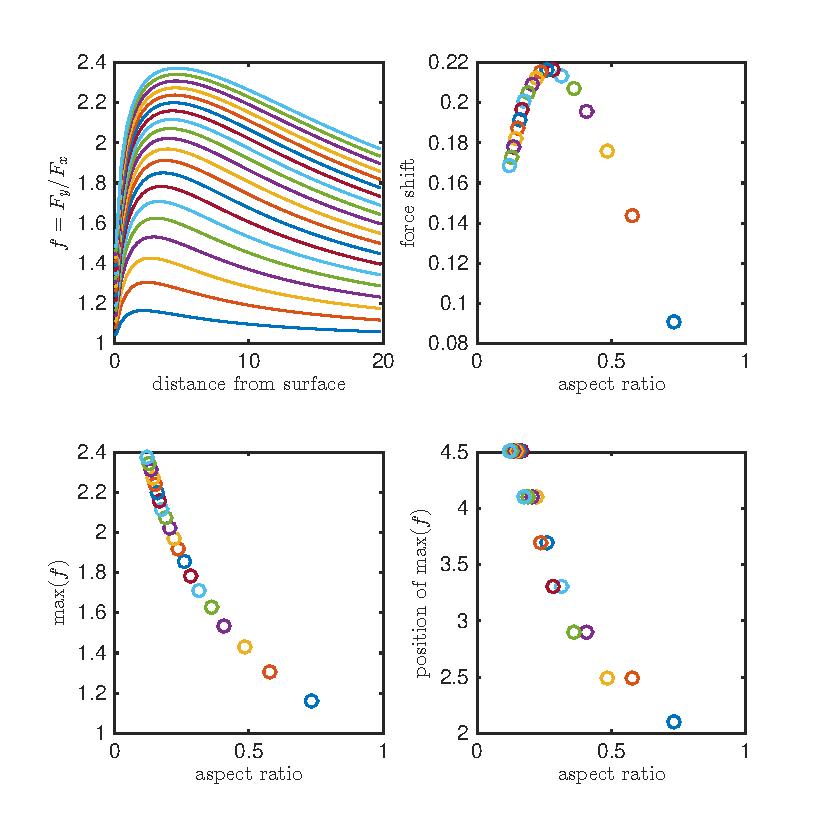
\includegraphics[scale=1,angle=0]{images/p2222}}
      \end{center}
\caption{ Interesting diagnostic quantities for the gravitational field around a squashed ellipse. The colour scheme between the panels is consistent. In the top-left panel we show the ratio $f$ of the force down the $x$- and $y$-axes as a function of distance from the surface; each colour corresponds to a different value of the aspect ratio of the ellipse. The actual values of the aspect ratios is given in the top-left panel, which shows the ``force shift''. This is the fractional difference between the maximum value of the force ratio, and the force ratio at the furthest distance from the surface shown. In the bottom-left panel we show the value of the maximum force ratio, as a function of the aspect ratio; in the bottom-right panel we show the position of the maximum force ratio. }\label{fig:squish-ellipse-grav}
\end{figure}

\subsubsection{Shapes via Legendre polynomials}
Creating a shape via
\bea
r(\theta) = \sum_{\ell=0}^n a_{\ell}P_{\ell}(\cos\theta)
\eea
In \tref{apple_coeffs} we give the values of the coefficients  $a_{\ell}$ required to generate the apple shape.
\begin{table}[!t]
\label{tab:priors}
\begin{center}
\begin{tabular}{|c|c|}  \hline 
Coefficient & Value \\ \hline 
$a_0$ & 0.3482169\\ \hline  
$a_1$ & 0.0969634 \\ \hline  
$a_2$ & -0.0450812 \\ \hline 
$a_3$ &  0.0346095\\ \hline 
$a_4$ & -0.0304927 \\ \hline  
$a_5$ &  0.0276200\\ \hline 
$a_6$ & -0.0245809\\ \hline 
$a_7$ & 0.0209728\\ \hline 
$a_8$ & -0.0168116\\ \hline  
$a_9$ & 0.0123419\\ \hline  
$a_{10}$ & -0.0079524\\ \hline  
$a_{11}$ & 0.0041198\\ \hline  
$a_{12}$ & -0.0013419\\ \hline   
\end{tabular}
\end{center}
\caption{Values of the coefficients in the Legendre expansion required to generate the ``apple'' shape.}
\label{apple_coeffs}
\end{table}%

\section{Comparisons to make}
Erect ``observation zone'' around an object; this is to be at a fixed location -- probably a circle surrounding the source. Then evaluate the force on that observation zone due to (a) chameleon, and (b) gravity. It may be easier to compute the forces due to the solutions to the linear and non-linear chameleon field equation. That is, numerically obtain the scalars $\phi$ and $\psi$ which solve
\bse
\bea
\nabla^2\phi &=&  \rho + m^2\left( \phi - \phi_{\infty}\right)- \tfrac{1}{\phi^2},\\
\nabla^2\psi &=&  \rho + m^2\left( \psi - \phi_{\infty}\right).
\eea
\ese
And then compute the forces due to each
\bea
\rbm{F}_{\phi} = - \nabla\phi,\qquad \rbm{F}_{\psi} = - \nabla\psi.
\eea
This will probe what effect the non-linearity $1/\phi^2$ has on the solutions, and therefore on the forces.
\section{Discussion}
 
\end{document}
